\documentclass[border=10pt]{standalone}
\usepackage[svgnames]{xcolor}
\usepackage{amsmath}
\usepackage{pgfplots}
\pgfplotsset{compat=newest}
\usepackage[sfdefault]{FiraSans}
\usepackage{FiraMono}
\renewcommand*\familydefault{\sfdefault}
\begin{document}
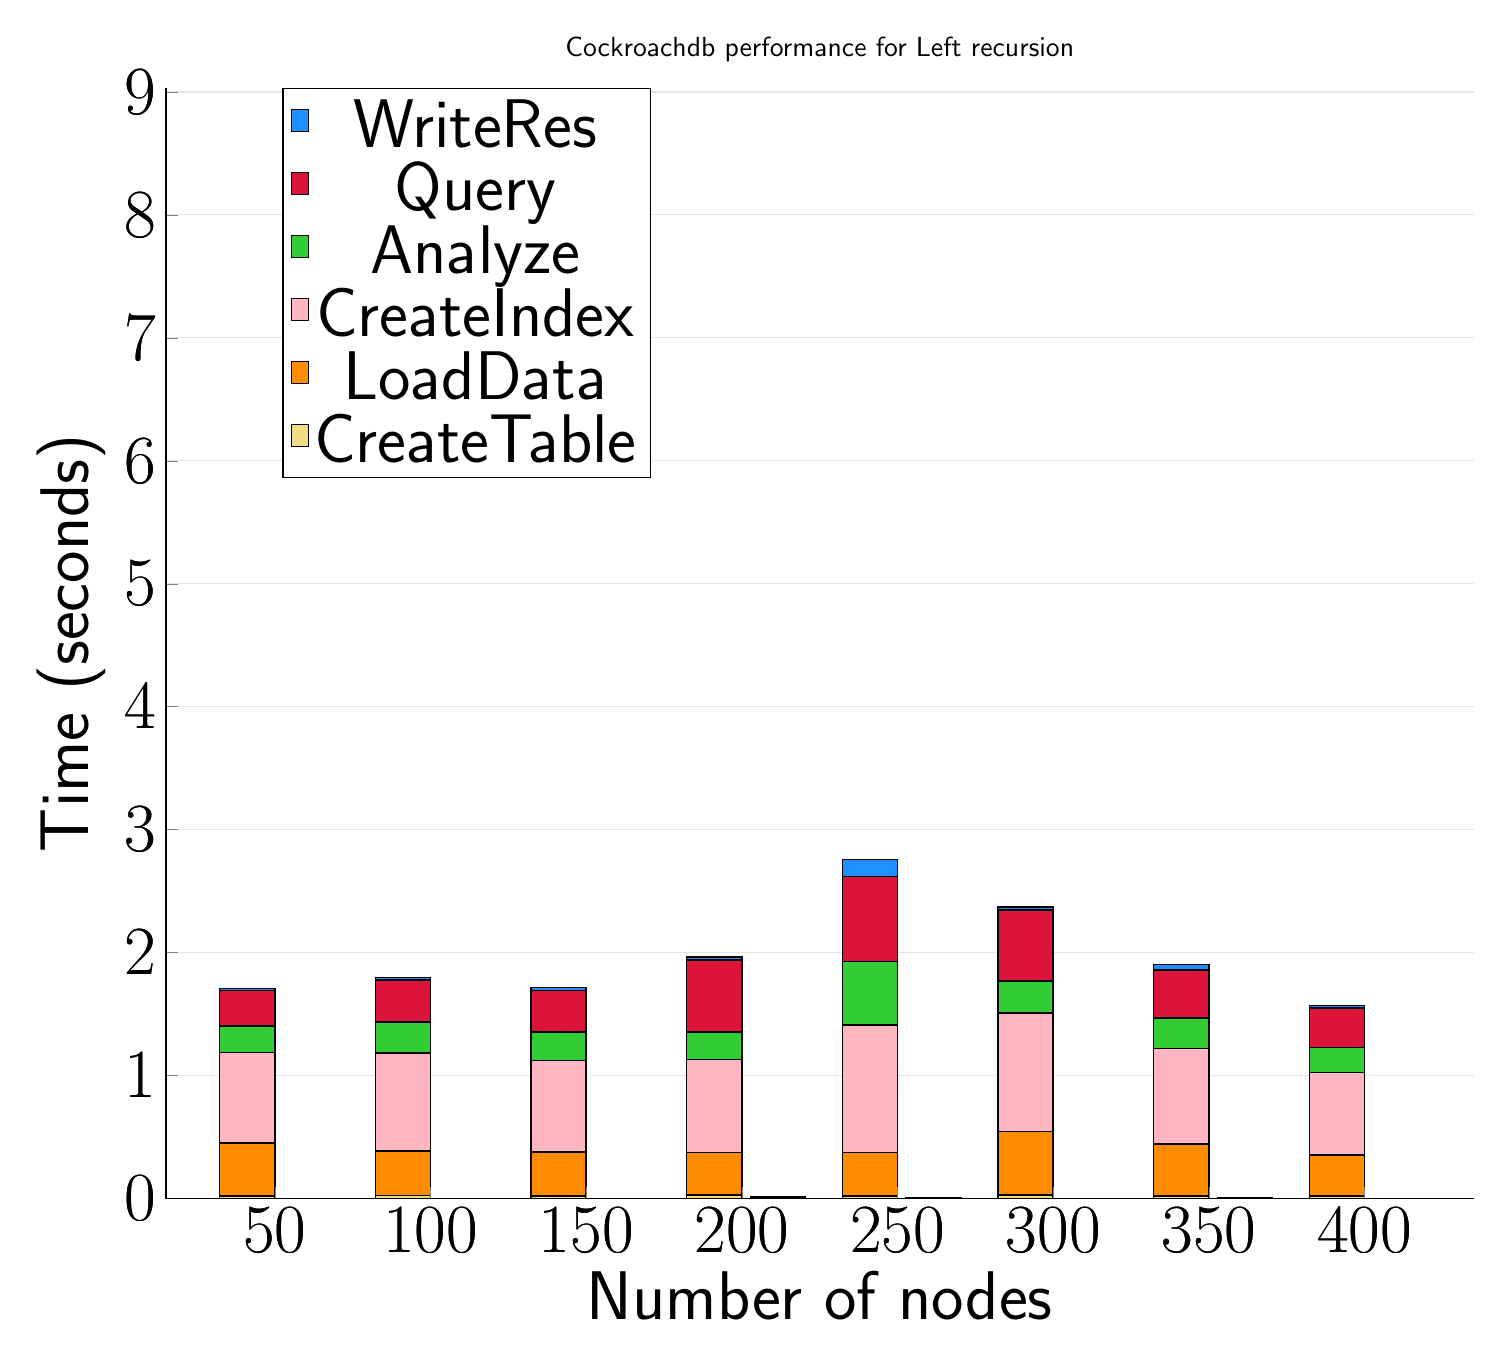
\begin{tikzpicture}
\begin{axis}[
   ybar stacked,
   title={Cockroachdb performance for Left recursion},
   bar shift=-10pt,
   width=1.5\textwidth,
   bar width=0.7cm,
   ymajorgrids, tick align=inside,
   major grid style={draw=gray!20},
   xtick=data,
   ymin=0, ymax=9.033333333830038,
   axis x line*=bottom,
   axis y line*=left,
   enlarge x limits=0.1,
   legend style={
       at={(0.23, 1)},
       anchor=north,
       legend columns=1,
       font=\Huge,
   },
   ylabel={Time (seconds)},
   xlabel={Number of nodes},
   label style={font=\Huge},
   tick label style={font=\Huge},
]
\addlegendimage{fill=DodgerBlue, draw=black, line width=0.2pt}
\addlegendentry{WriteRes}
\addlegendimage{fill=Crimson, draw=black, line width=0.2pt}
\addlegendentry{Query}
\addlegendimage{fill=LimeGreen, draw=black, line width=0.2pt}
\addlegendentry{Analyze}
\addlegendimage{fill=LightPink, draw=black, line width=0.2pt}
\addlegendentry{CreateIndex}
\addlegendimage{fill=DarkOrange, draw=black, line width=0.2pt}
\addlegendentry{LoadData}
\addlegendimage{fill=LightGoldenrod, draw=black, line width=0.2pt}
\addlegendentry{CreateTable}
\addplot +[fill=LightGoldenrod, draw=black, line width=0.5pt] coordinates {
    (50, 0.019999998311201733)
    (100, 0.023333333432674408)
    (150, 0.019999998311201733)
    (200, 0.02999999870856603)
    (250, 0.020000000794728596)
    (300, 0.030000001192092896)
    (350, 0.019999998311201733)
    (400, 0.020000000794728596)
};
\addplot +[fill=DarkOrange, draw=black, line width=0.5pt] coordinates {
    (50, 0.4333333323399226)
    (100, 0.3633333345254262)
    (150, 0.36000000188748044)
    (200, 0.3466666688521703)
    (250, 0.3566666642824809)
    (300, 0.5166666681567827)
    (350, 0.4233333319425583)
    (400, 0.3333333358168602)
};
\addplot +[fill=LightPink, draw=black, line width=0.5pt] coordinates {
    (50, 0.7333333343267441)
    (100, 0.7966666668653488)
    (150, 0.7433333347241083)
    (200, 0.7566666677594185)
    (250, 1.0333333338300388)
    (300, 0.9633333310484886)
    (350, 0.7766666660706202)
    (400, 0.6699999993046125)
};
\addplot +[fill=LimeGreen, draw=black, line width=0.5pt] coordinates {
    (50, 0.2166666661699613)
    (100, 0.25333333263794583)
    (150, 0.2299999992052714)
    (200, 0.2199999988079071)
    (250, 0.5199999983112017)
    (300, 0.26000000288089115)
    (350, 0.2500000024835269)
    (400, 0.20333333065112433)
};
\addplot +[fill=Crimson, draw=black, line width=0.5pt] coordinates {
    (50, 0.2866666664679845)
    (100, 0.3400000010927518)
    (150, 0.3400000010927518)
    (200, 0.586666668454806)
    (250, 0.690000000099341)
    (300, 0.5766666630903879)
    (350, 0.38999999811251956)
    (400, 0.32333333293596905)
};
\addplot +[fill=DodgerBlue, draw=black, line width=0.5pt] coordinates {
    (50, 0.020000000794728596)
    (100, 0.023333333432674408)
    (150, 0.02333333094914754)
    (200, 0.02333333094914754)
    (250, 0.13666666795810065)
    (300, 0.023333335916201275)
    (350, 0.04333333174387614)
    (400, 0.020000003278255463)
};
\end{axis}
\begin{axis}[
   ybar stacked,
   bar shift=13pt,
   width=1.5\textwidth,
   bar width=0.7cm,
   ymajorgrids, tick align=inside,
   major grid style={draw=none},
   xtick=data,
   ymin=0, ymax=9.033333333830038,
   axis x line*=none,
   axis y line*=none,
   enlarge x limits=0.1,
   label style={font=\Huge},
   tick label style={font=\Huge},
]
\addplot +[fill=LightGoldenrod, draw=black, line width=0.5pt] coordinates {
    (50, 0.0)
    (100, 0.0)
    (150, 0.0)
    (200, 0.006666666666666672)
    (250, 0.0066666666666666706)
    (300, 0.0)
    (350, 0.0)
    (400, 0.0)
};
\addplot +[fill=DarkOrange, draw=black, line width=0.5pt] coordinates {
    (50, 0.0)
    (100, 0.0)
    (150, 0.0)
    (200, 0.0)
    (250, 0.0)
    (300, 0.0)
    (350, 0.006666666666666668)
    (400, 0.0)
};
\addplot +[fill=LightPink, draw=black, line width=0.5pt] coordinates {
    (50, 0.0)
    (100, 0.0)
    (150, 0.0)
    (200, 0.0)
    (250, 0.0)
    (300, 0.0)
    (350, 0.0)
    (400, 0.0)
};
\addplot +[fill=LimeGreen, draw=black, line width=0.5pt] coordinates {
    (50, 0.0)
    (100, 0.0)
    (150, 0.0)
    (200, 0.0)
    (250, 0.0)
    (300, 0.0)
    (350, 0.0)
    (400, 0.0)
};
\addplot +[fill=Crimson, draw=black, line width=0.5pt] coordinates {
    (50, 0.0)
    (100, 0.0)
    (150, 0.0)
    (200, 0.0066666666666666706)
    (250, 0.0)
    (300, 0.0)
    (350, 0.0)
    (400, 0.0)
};
\addplot +[fill=DodgerBlue, draw=black, line width=0.5pt] coordinates {
    (50, 0.0)
    (100, 0.0)
    (150, 0.0)
    (200, 0.0)
    (250, 0.0)
    (300, 0.0)
    (350, 0.003333333333333336)
    (400, 0.0)
};
\end{axis}
\end{tikzpicture}

\end{document}
